%!TEX TS-program = xelatex
%!TEX root = ../../maxwell2018thesis.tex

\chapter[A Background of Stopping in IIR]{A Background of Stopping in\\Interactive Information Retrieval}\label{chap:stopping_background}

In the previous chapter, we provided a high level overview of~\gls{acr:ir}. In particular, we provided a brief history of the area, the basic families of retrieval models, and various measures that have traditionally been used to evaluate the effectiveness of a retrieval system. Towards the end of the chapter, we began to shift from the \emph{system-sided} research that has dominated~\gls{acr:ir} research (and quite understandably so), towards the more \emph{user-centred} research with which the work in this thesis considers. In particular, as alluded to in Chapter~\ref{chap:intro}, and indeed in the title of this thesis, we now turn our attention to the concept of \emph{stopping behaviour} in the context of~\gls{acr:iir}.

\begin{figure}[h]
    \centering
    \vspace{4mm}
    \resizebox{1\hsize}{!}{
    
\includegraphics{figures/ch3-stopsign.pdf}}
    \label{fig:stopsign}
    \vspace{-5mm}
\end{figure}

With many of the models and measures employed in~\gls{acr:ir} and~\gls{acr:iir} research today largely agnostic of a searcher's stopping behaviour, we in this chapter provide an overview of a variety of different \emph{stopping heuristics} that have been defined in the literature over a number of decades, provide a discussion on a number of different user studies that have examined searcher stopping behaviours, discuss basic theoretical frameworks that provide a potential insight and explanation into why people stop, and then discuss a variety of different user models that have been developed that better attempt to model a searcher's interactions, and thus allow for a better representation of their stopping behaviour.

\section{Why Stopping?}
\todo{This is lifted from the introduction chapter. Where does it fit better? Would a shorter form of this in the introduction  be better?} Knowing when to stop is a fundamental aspect of human thinking, with individuals commonly employing some form of \emph{stopping criterion} to decide when they should stop with their interactions in the world around them~\citep{nickles1995judgment}. As an example, a shopper looking to buy a new smartphone will stop shopping around once he or she has obtained sufficient information on what new device to purchase. A doctor, once their case notes about a patient's condition have been finished, will then diagnose their ailment. In the context of search, stopping may be considered at a variety of different points during the search process. The commonly used example of \emph{search stopping behaviour} is the point at which a searcher should stop examining a list of ranked results, or, in other words, \emph{how far down the ranked list the searcher should go}, for example.

The decision of when to stop is not necessarily due to external factors, but from a series of \emph{internal factors} of the decision maker's thinking process. In the context of informational search, knowing when to stop requires that the individual makes a judgement regarding the sufficiency of the information obtained, and whether or not additional information is required to be obtained~\citep{browne2004stopping_rules}. This is normally characterised by both the completeness and correctness of the information obtained thus far~\citep{smith1991belief}. These claims can be mirrored by qualitative studies on examining stopping behaviour, where researchers have found that searchers stop examining a ranked list of results simply because what they have found previously is \emph{``good enough''}~\citep{wu2014information_scent}.

\section{Stopping Heuristics}\label{sec:stopping_background:heuristics}
Considering the above explanation, researchers have devised a series of different high level \emph{stopping heuristics} as a means to try and encapsulate the sense of what is \emph{``good enough''} entails. These heuristics have been defined primarily in information science, although as we proceed through the chapter, fields such as ecology will also be shown to contain stopping rules that can be applied directly to the process of search.

It should be noted that in the context of search, two key \emph{stopping decision points} are often mooted in the literature concerning when a searcher should stop. Figure~\ref{fig:model_two_points} illustrates an excerpt from a user model, illustrating these two points: decision point \blueboxbold{1} considers \emph{snippet level stopping} -- often referred to as \emph{query level stopping} in the literature. The second stopping decision point \blueboxbold{2} considers wider \emph{session level stopping}. While these stopping decision points are discussed in detail in Section~\ref{sec:proposal:stopping_points}, it should be noted that the heuristics defined in this section can be applied to snippet level stopping, session level stopping, or both.

\begin{figure}[t!]
    \centering
    \resizebox{1\hsize}{!}{
    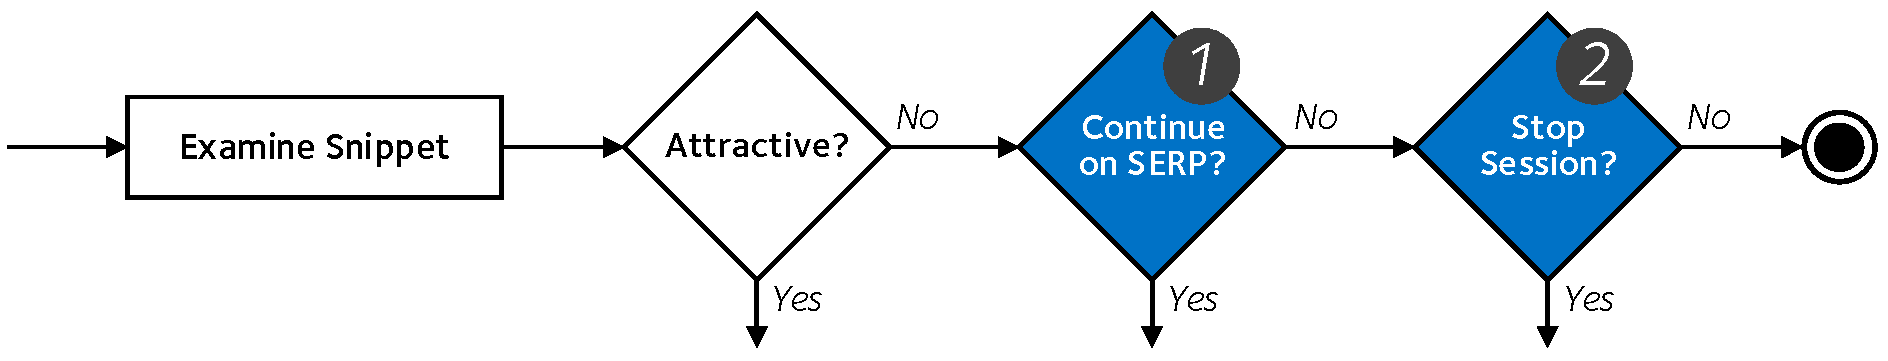
\includegraphics{figures/ch3-two_points.pdf}}
    \caption[Two main stopping decision points of the search process]{An excerpt from a wider user search model, demonstrating two key, established stopping decision points commonly discussed in the literature. These are highlighted in the illustration as {\color{dmax_lightblue}blue} diamonds. The two points consider \blueboxbold{1} \emph{snippet level stopping} (often called \emph{query level stopping}), and \blueboxbold{2} \emph{session level stopping}.}
    \label{fig:model_two_points}
\end{figure}

\subsection{Satisfaction and Frustration}
Two of the earliest stopping heuristics defined in the literature are by~\cite{cooper1973retrieval_effectiveness_ii}, who devised two stopping heuristics as a means for estimating the utility a searcher can attain when interacting with a system. While the means of which~\cite{cooper1973retrieval_effectiveness_ii} estimated the utility of search are not of key relevance to this thesis, the work on stopping heuristics are. The \emph{satisfaction point} and \emph{frustration point} stopping heuristics were defined, considering a searcher's perceived satisfaction and tolerance to non-relevance, respectively.

\subsubsection{Satisfaction}
Given the name, it is not surprising that the \emph{satisfaction point} rule considers the point at which a searcher has found enough perceived relevant material to consider his or her search a success. It can be easily imagined that such a rule would apply directly to both snippet level stopping (i.e. \emph{find $x$ relevant documents on this SERP}) and session level stopping (i.e. \emph{find $x$ relevant documents}).

\subsubsection{Frustration}
In a converse fashion to the satisfaction point heuristic, the \emph{frustration point} heuristic considers a searcher's overall \emph{tolerance to non-relevance}, by stopping after being sufficiently frustrated by the results presented to our searcher.

\subsubsection{Repetition and Combining Heuristics}
The two relatively straightforward heuristics defined above makes a searcher's interactions with a ranked list of results, or SERPs, \emph{inherently adaptive.} Given a set of results, his or her behaviour will change with respect to the perceived quality of the ranked list of results. As a reminder, this would not necessarily mean considering the system's effectiveness measures, but rather user-focused measures such as interactive precision and recall (refer to Section~\ref{sec:ir_background:user:evaluation:interactive_pr}).

Perhaps due to the relative simplicity of these heuristics, identical approaches have also been defined elsewhere in the literature.~\cite{kraft1979stopping_rules} later defined three further stopping heuristics, two of which are the \emph{satiation} and the somewhat loaded \emph{disgust} heuristics. These essentially are the satisfaction and disgust heuristics as previously defined by~\cite{cooper1973retrieval_effectiveness_ii}. Within the satiation rule, a searcher will stop after been \emph{satiated} by finding a number of documents considered to be relevant, while the disgust rule considers a searcher's disgust at finding a number of non-relevant documents.

\cite{kraft1979stopping_rules} also proposed a third heuristic that \emph{combines} both the satisfaction/satiation and frustration/disgust rules together into a single heuristic. Here, a searcher following such an approach would be inclined to stop examining content if they were either satisfied with what had been found, or disgusted by having to trawl through a number of material judged to be non-relevant. The stopping point would be whatever of the two conditions are met first. Indeed,~\cite{kraft1979stopping_rules} demonstrated that the expected search length of a searcher could be approximated using each of the two stopping heuristics by considering the size of the retrieval set, the number of relevant documents a searcher wished to obtain, and the number of non-relevant documents a searcher would be willing to tolerate. The number of documents required to consider a search as successful is dependent upon whether the search task is high precision (where one would stop comparatively early), or high recall (where one would stop comparatively later), as hypothesised by~\cite{bates1984thirty_items}.

\subsection{Mental List}

\subsection{Representational Stability}

\subsection{Difference Threshold}

\subsection{Magnitude Threshold}

\subsection{The Single Criterion}

\subsection{Summary of Heuristics}
covered a number of different heuristics.
of course, these heuristics will not always be applicable to certain contexts...

\section{User Studies}

\section{Models of Search}
From more conceptual, to theoretical.

\subsection{Search Economic Theory}

\section{Information Foraging Theory}

\subsection{Conceptual Models}

\begin{figure}[t!]
    \centering
    \resizebox{1\hsize}{!}{
    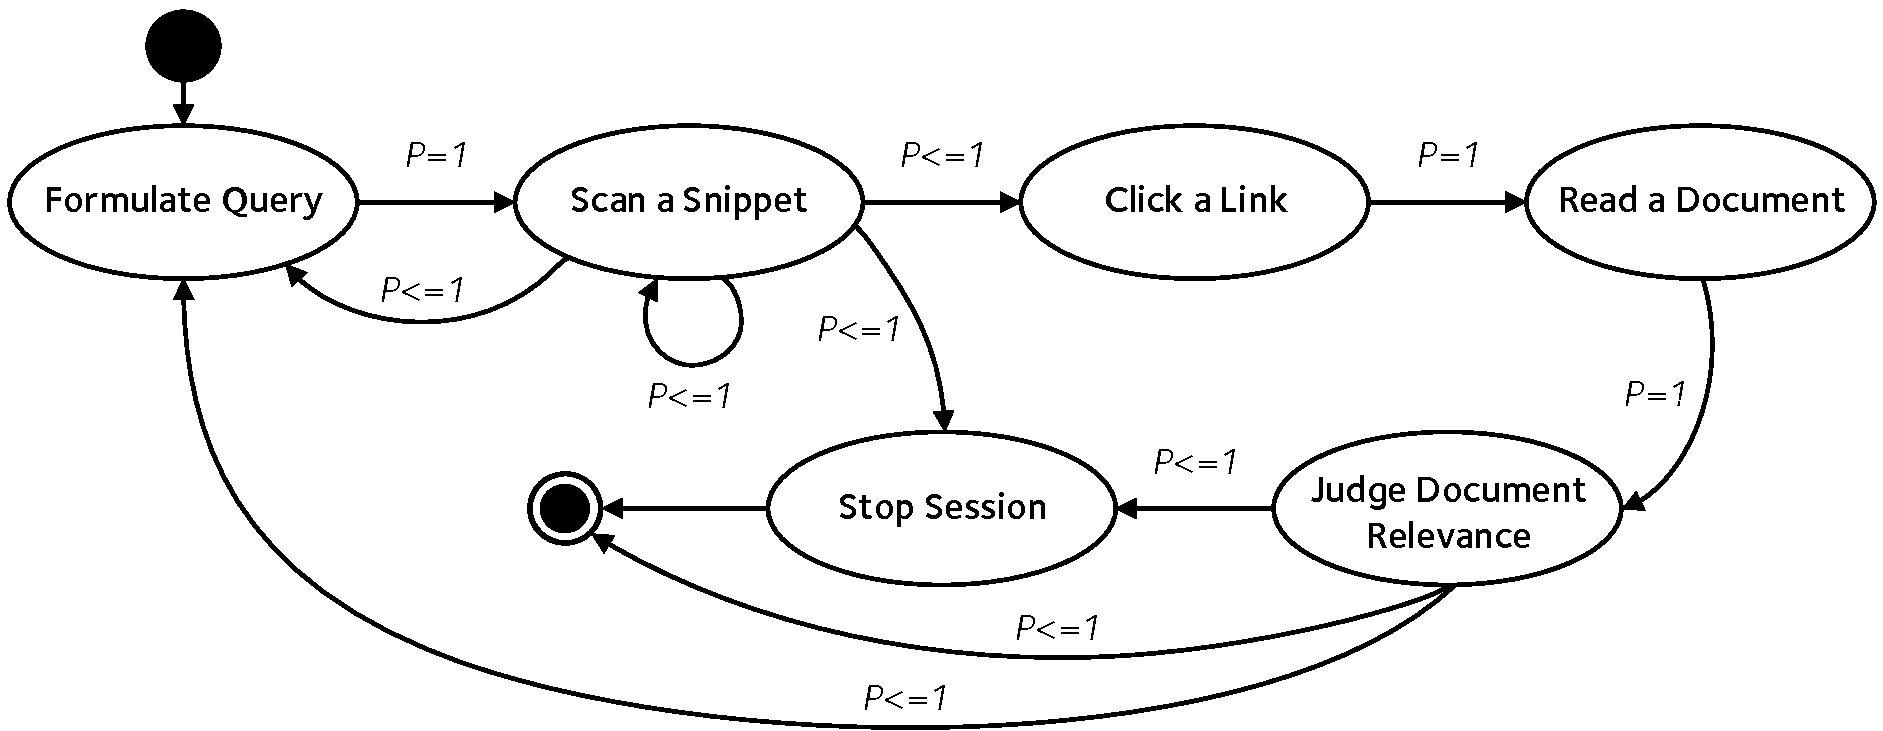
\includegraphics{figures/ch3-baskaya.pdf}}
    \caption[Model of the search process by~\cite{baskaya2013behavioural_factors}]{The user model of search, as outlined by~\citealt{baskaya2013behavioural_factors}. Represented as a Markov Model, the model considers six steps in all. Encoded within two of the steps are decision points that a user following this model must consider in order to continue. Figure adapted (with permission) from the authors of~\citealt{baskaya2013behavioural_factors}.}
    \label{fig:baskaya_model}
\end{figure}

\begin{figure}[t!]
    \centering
    \resizebox{1\hsize}{!}{
    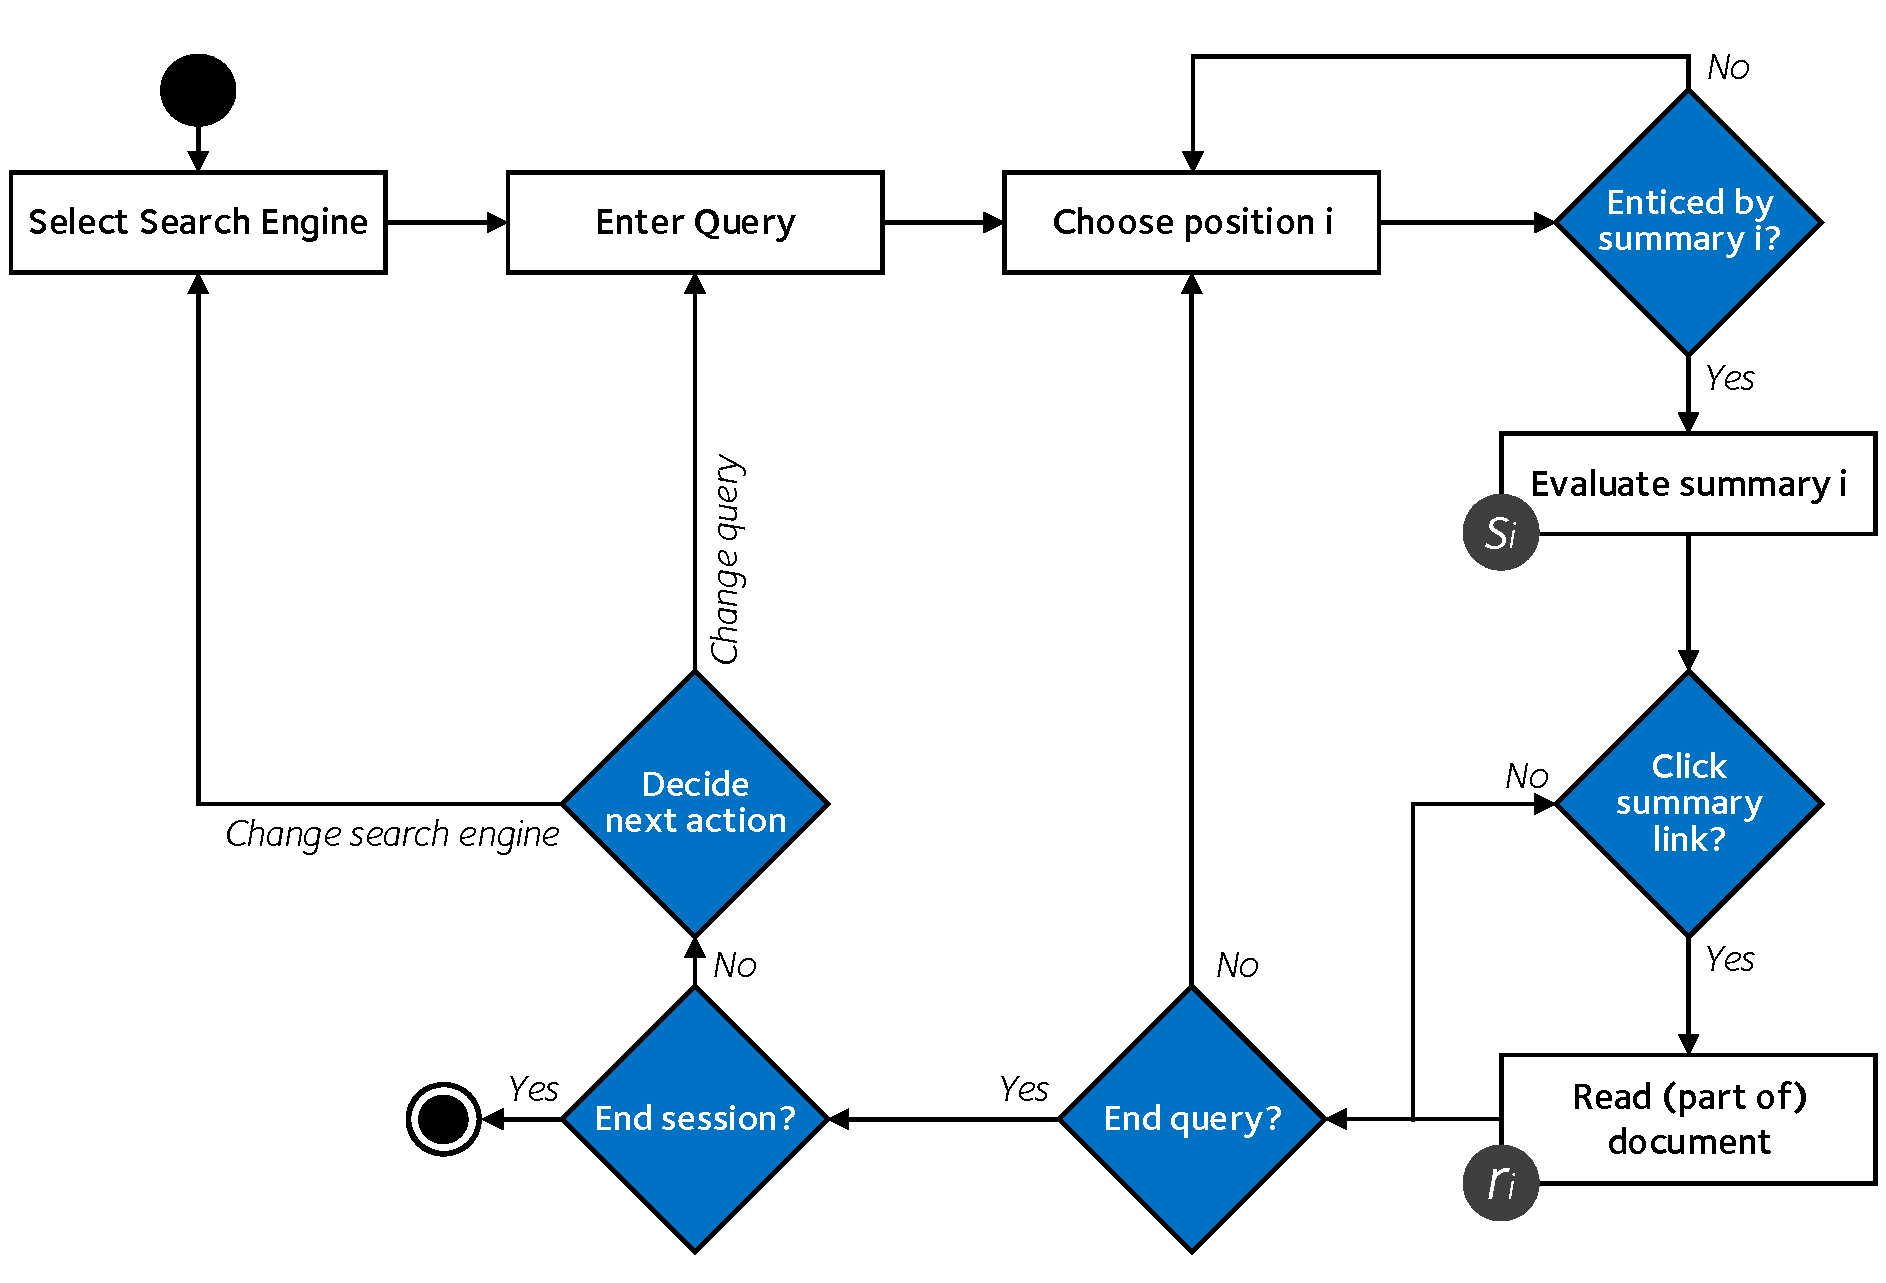
\includegraphics{figures/ch3-thomas.pdf}}
    \caption[Model of the search process by~\cite{thomas2014modelling_behaviour}]{A model of the search process, considering the high-level processes undertaken by a searcher, as outlined by~\cite{thomas2014modelling_behaviour}. Also included are a number of decision points (represented as diamonds) that searchers must consider when following this model. Figure adapted (with permission) from the authors of~\citealt{thomas2014modelling_behaviour}. \textcopyright~Paul Thomas, Peter Bailey, Alistair Moffat and Falk Scholer.}
    \label{fig:thomas_model}
\end{figure}

\subsubsection{Carterette}

\subsubsection{Baskaya}

\subsubsection{Thomas}

\subsubsection{Vu}

\section{Chapter Summary}

% - given you an outline of the basics of IR
% - and more system-sided IR
%
% - including a discussion on some of the various measures that are used
% - still very naive in terms of \emph{stopping behaviour}. i.e. assume fixed depths, typically naive about relevance.
%
% - so in this chapter, we begin to consider things from the central point of this thesis - stopping during search.
%
%
%
% - to this end, we in this chapter discuss:
%
% - a variety of different stopping heuristics
% - discuss the basic theories that can be used to explain one's stopping behaviour;
% - and explain the results from different user studies examining a searcher's stopping behaviour
%
% - we then take time to examine
%
% - some of the more complex models of search which are better able to capture stopping.
% 
% \section{Stopping Heuristics}\label{sec:stopping_background:heuristics}
%
% \section{User Studies}
% ryen white's expert stuff -- does he report stopping stuff?
%
% depth first vs breadth first??
%
% conceptual models (e.g. following on from TREC, we end up with...thomas, baskaya...), then move on to theoretical models
%
% like we mentioned in Ch2, in the different measures, we have different stopping rules encoded within them.
% e.g. Carterette's 2011 model.
%
% \section{Models of Search}
%
% \subsection{Conceptual Models}
% The Berry Picking Model
%
% \begin{figure}[t!]
%     \centering
%     \resizebox{1\hsize}{!}{
%     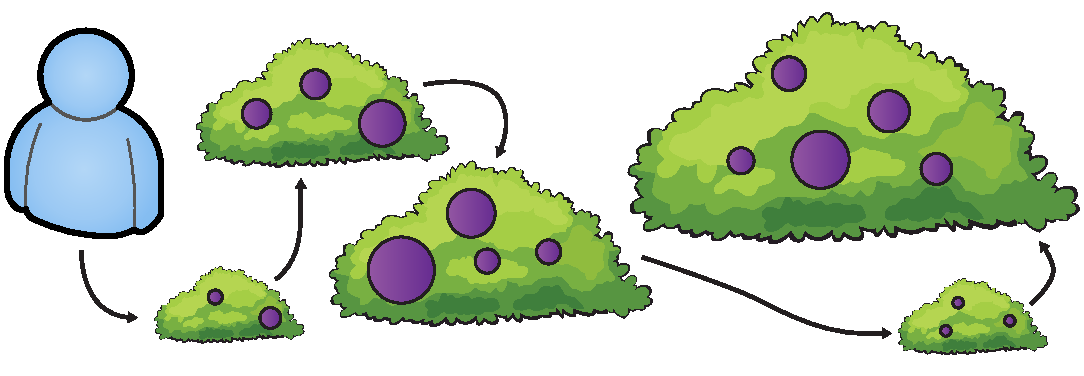
\includegraphics{figures/ch3-berry_picking.pdf}}
%     \caption[The Berry Picking Model~\cite{bates1989berry_picking}]{The Berry Picking Model, defined by~\citealt{bates1989berry_picking}.}
%     \label{fig:berry_picking}
% \end{figure}
%
%
% \subsection{Information Foraging Theory}
%
% \subsection{(Interactive) Probability Ranking Principle}
%
% \subsection{Search Economic Theory}
%
% \subsection{Simple TREC User Model}
%
% \subsection{Paul Thomas Model}
%
% \subsection{Feza Model}
%
% Need to illustrate that there is a development of the user model here.
%
% What about the attention model in ``Beyond ten blue links: enabling user click modeling in federated web search''?
%
% \begin{figure}[t!]
%     \centering
%     \resizebox{1\hsize}{!}{
%     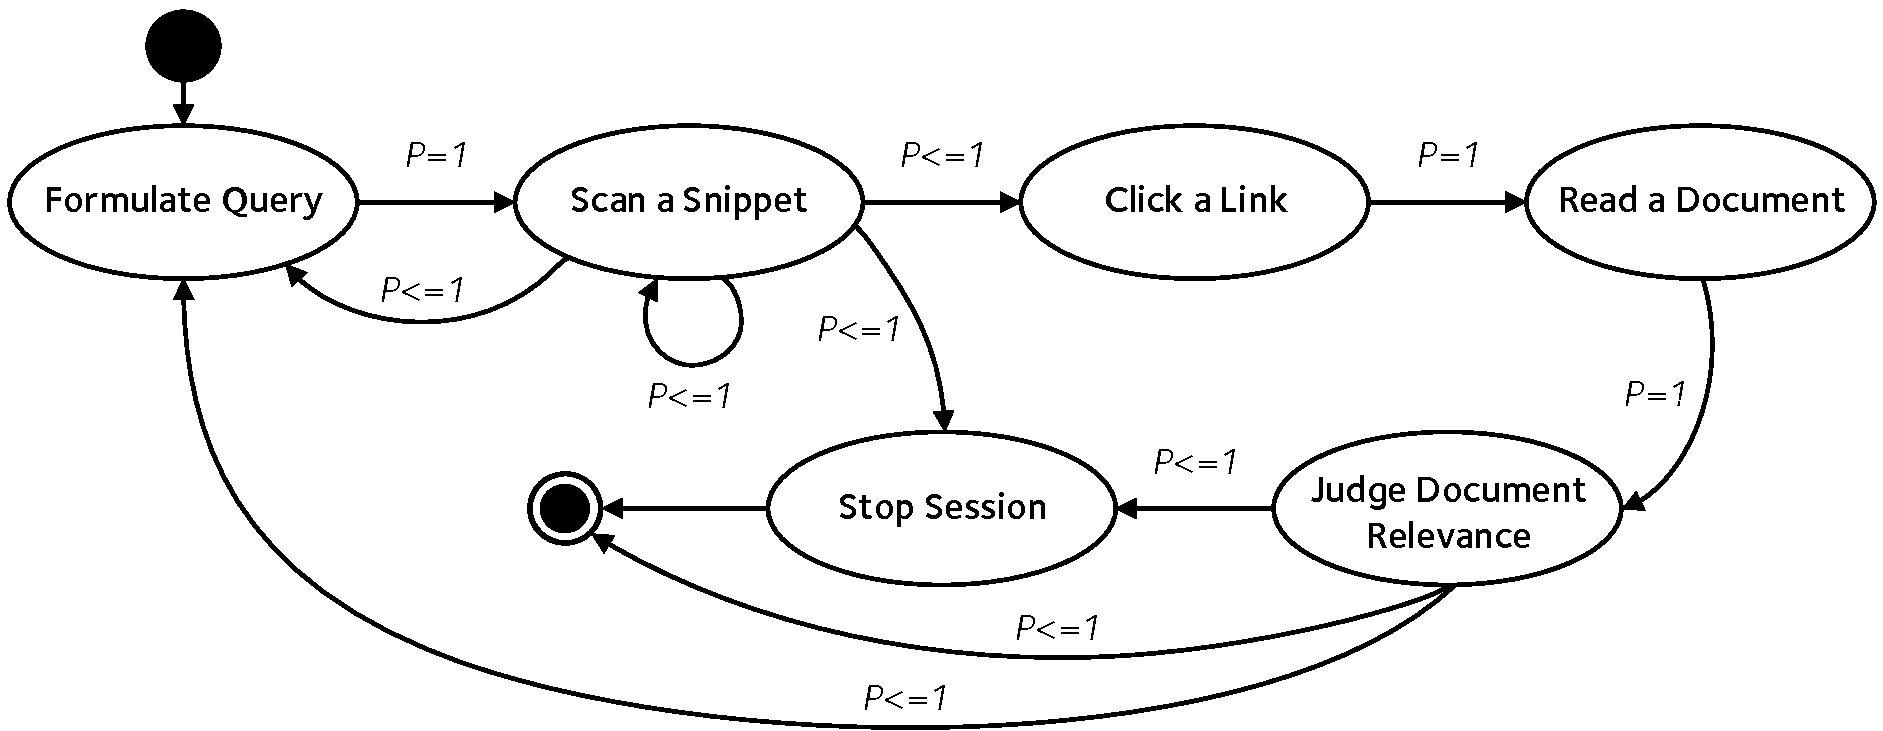
\includegraphics{figures/ch3-baskaya.pdf}}
%     \caption[Model of the search process by~\cite{baskaya2013behavioural_factors}]{The user model of search, as outlined by~\citealt{baskaya2013behavioural_factors}. Represented as a Markov Model, the model considers six steps in all. Encoded within two of the steps are decision points that a user following this model must consider in order to continue. Figure adapted (with permission) from the authors of~\citealt{baskaya2013behavioural_factors}.}
%     \label{fig:baskaya_model}
% \end{figure}
%
% \begin{figure}[t!]
%     \centering
%     \resizebox{1\hsize}{!}{
%     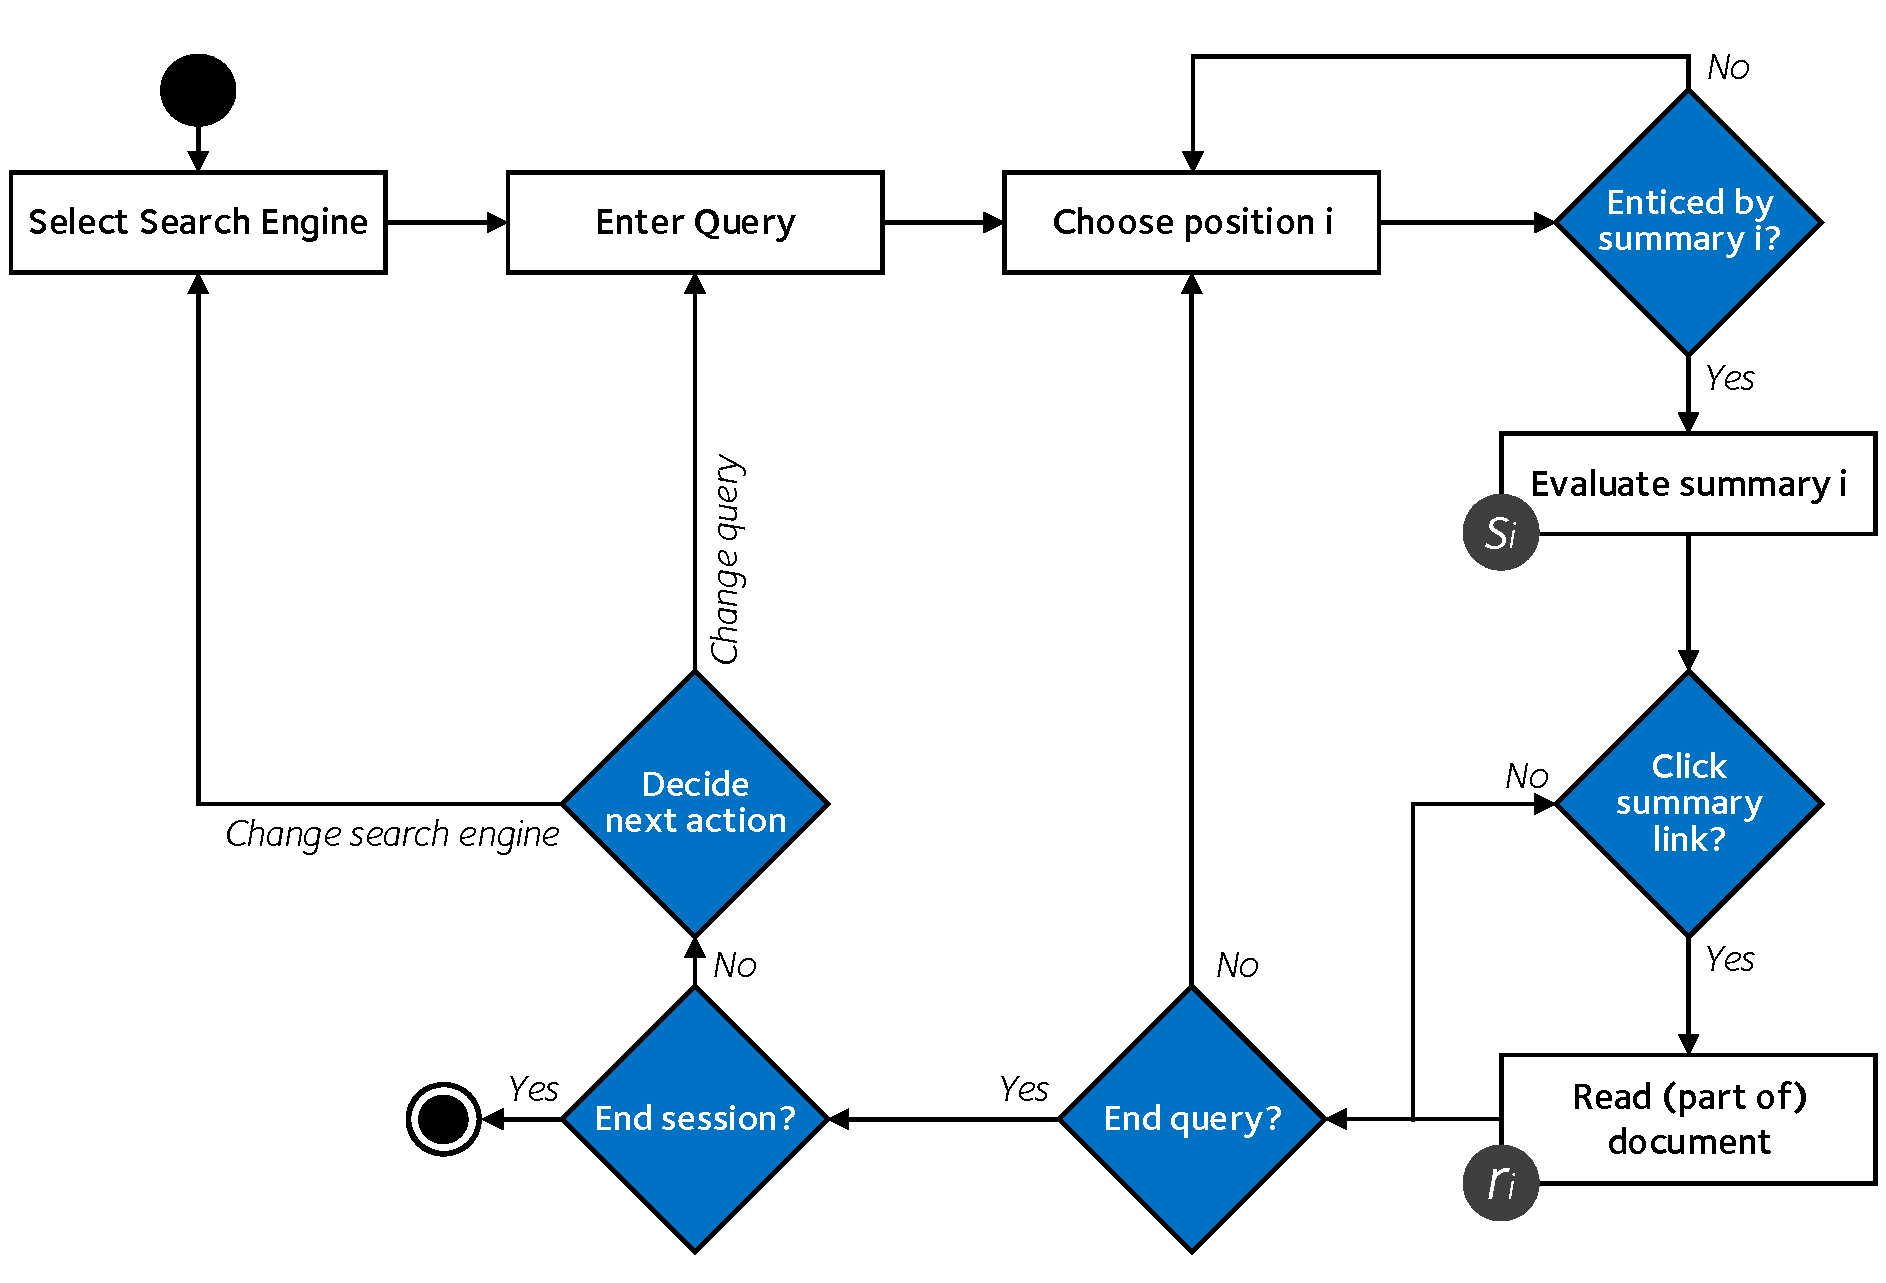
\includegraphics{figures/ch3-thomas.pdf}}
%     \caption[Model of the search process by~\cite{thomas2014modelling_behaviour}]{A model of the search process, considering the high-level processes undertaken by a searcher, as outlined by~\cite{thomas2014modelling_behaviour}. Also included are a number of decision points (represented as diamonds) that searchers must consider when following this model. Figure adapted (with permission) from the authors of~\citealt{thomas2014modelling_behaviour}. \textcopyright~Paul Thomas, Peter Bailey, Alistair Moffat and Falk Scholer.}
%     \label{fig:thomas_model}
% \end{figure}
%
%
% Refer to the following chapter for more information on how we extend these models to make them more realistic.
%
